\documentclass[conference]{IEEEtran}
\IEEEoverridecommandlockouts
% The preceding line is only needed to identify funding in the first footnote. If that is unneeded, please comment it out.
\usepackage[ngerman]{babel}
\usepackage{cite}
\usepackage{amsmath,amssymb,amsfonts,mathtools}
\usepackage{algorithmic}
\usepackage{graphicx}
\usepackage{textcomp}
\usepackage[dvipsnames]{xcolor}
\def\BibTeX{{\rm B\kern-.05em{\sc i\kern-.025em b}\kern-.08em
    T\kern-.1667em\lower.7ex\hbox{E}\kern-.125emX}}
\usepackage{listings}
\usepackage{tabularx}
\usepackage{booktabs}
\usepackage{siunitx}
\usepackage{float}
\usepackage{caption}

\definecolor{codegreen}{rgb}{0,0.6,0}
\definecolor{codegray}{rgb}{0.5,0.5,0.5}
\definecolor{codepurple}{rgb}{0.58,0,0.82}
\definecolor{backcolour}{rgb}{0.95,0.95,0.95}
\renewcommand{\lstlistingname}{Code}% Listing -> Algorithm
\renewcommand{\lstlistlistingname}{List of \lstlistingname s}% List of Listings -> List of Algorithms
\lstdefinestyle{mystyle}{
    backgroundcolor=\color{backcolour},
    commentstyle=\color{codegreen},
    keywordstyle=\color{magenta},
    numberstyle=\tiny\color{codegray},
    stringstyle=\color{codepurple},
    basicstyle=\ttfamily\footnotesize,
    breakatwhitespace=false,
    breaklines=true,
    captionpos=b,
    keepspaces=true,
    numbers=left,
    numbersep=3pt,
    showspaces=false,
    showstringspaces=false,
    showtabs=false,
    tabsize=3
}
\lstset{style=mystyle}

\usepackage{hyperref}
\hypersetup{
    pdftex,
    pdftitle={Versuch ASM},
    pdfsubject={Versuch ASM},
    pdfauthor=AJC,
    colorlinks,
    citecolor=black,
    filecolor=black,
    linkcolor=black,
    urlcolor=black
}



\begin{document}

\title{
    \centering
    
\includegraphics[width=0.5\textwidth]{../OTHR_OTHR_Logo.pdf}\\
    \textsc{Drehstrom-Asynchronmaschine mit Schleifringläufer} \\
}

\maketitle\\

\begin{abstract}
    In diesem Versuch soll eine Asynchronmaschine mit Schleifringläufer genauer
    untersucht werden. Die Versuchsmaschine wird mithilfe einer
    Käfigläufer-Asynchronmaschine belastet, deren Drehzahl mithilfe eines
    Frequenzumrichters gesteuert werden kann. \\
    Zur Bestimmung der Ersatzschaltbild-Parameter werden ein Kurzschluss- und ein 
    Leerlaufversuch durchgeführt. Der Kurzschlussversuch dient der Bestimmung der Parameter im
    Längszweig, des komplexen Anlaufstromes sowie des Anzugmomentes. Mithilfe
    des Leerlaufversuches lassen sich die Parameter im Querzweig und der
    komplexe Leerlaufstrom bestimmen. Dazu wird die Ständerspannung verändert.\\
    Im nächsten Versuchsteil wird die Belastung der ASM und die synchrone
    Drehzahl untersucht. Die Messungen werden im Betriebsbereich um die
    synchrone Drehzahl aufgenommen, damit die Belastung der Maschine im
    motorischen und generatorischen Betrieb gemessen werden kann.\\
    Im letzten Versuchsteil wird die im Schleifringläufer induzierte Spannung in
    Abhängikeit zur Drehzahl gemessen.

\end{abstract}

\section{Anlaufmoment und Kippmoment}

Bei diesem Versuch wurde das Drehmoment mit einem 40cm langen Stab und einer
Digitalen Wage gemessen.

Mit der Gleichung \ref{eq:moment} wurde das Drehmoment aus den Messungen berechnet.

\begin{equation} \label{eq:moment}
    M=G\cdot g\cdot l = \frac{G(I_1)}{1000}\si{kg}\cdot 9,81\si{m/s^2} \cdot 0,4\si{m}
\end{equation}

In den Abbildungen \ref{fig:Anlaufmoment} und \ref{fig:Kippmoment} wird das
Anlaufmoment der ASM über die Spannung graphisch dargestellt.

Die obere Hälfte der Abbildungen zeigt eine linearisierte Extrapolation des
Verlaufs der Drehmomente $M_{an}$ und $M_{\textit{Kipp}}$ über die Spannung
$U_1^2$, bis $400^2V$.

Aber in der unteren Hälfte der Abbildungen wird das Drehmoment der ASM direkt
über die Spannung $U_1$ dargestellt und mit einer quadratischen Polynomfunktion
extrapoliert.

\begin{table}[htbp]
    \centering
    \begin{tabularx}{\columnwidth}{XXXXXXX}
    \toprule
     $I_1[A]$ &  $P_1[W]$ &  $U[V]$ &  $G[g]$ &  $M_{an}[Nm]$ \\
    \midrule
            1,0 &          28 &      27,5 &        35 &        0,137340 \\
            2,0 &          92 &      55,0 &        85 &        0,333540 \\
            3,0 &         194 &      82,0 &       222 &        0,871128 \\
            4,0 &         352 &     107,0 &       426 &        1,671624 \\
            4,2 &         392 &     113,0 &       464 &        1,820736 \\
            5,0 &         470 &     134,0 &       685 &        2,687940 \\
    \bottomrule
    \end{tabularx}
    \caption{Anlaufmoment}
\end{table}


\begin{figure}[htbp]
    \centering
    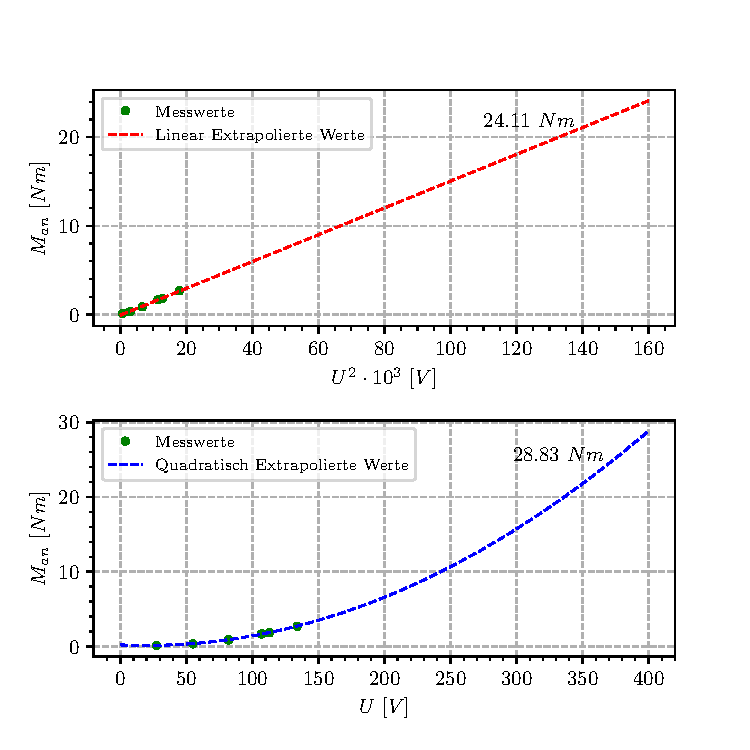
\includegraphics[width=\columnwidth]{./figures/anlaufmoment.pdf}
    \caption{Anlaufmoment}
    \label{fig:Anlaufmoment}
\end{figure}

Der lineare Verlauf in Abb.\ref{fig:Anlaufmoment}, $M_{an}(U)$ [\textcolor{red}{rot}]:
\begin{gather*}
    0,1511 x - 0,07306 \\
    M_{an}(U_N=400^2V^2)=24,11\ \si{Nm}
\end{gather*}

Und die quadratische Polynomfunktion $M_{an}(U)$ [\textcolor{blue}{blau}]:
\begin{gather*}
    0,000199 x^2 -0,007889 x + 0,190977\\
    M_{an}(U_N=400V)=28,83\ \si{Nm}
\end{gather*}

\begin{table}[htbp]
    \centering
    \begin{tabularx}{\columnwidth}{XXXXXXX}
        \toprule
             $I_1[A]$ &  $P_1[W]$ &  $U[V]$ &  $G[g]$ &  $M_{an}[Nm]$ \\
        \midrule
                1,0 &          24 &        36 &        32 &        0,125568 \\
                2,0 &         102 &        73 &       218 &        0,855432 \\
                3,0 &         380 &       108 &       508 &        1,993392 \\
                4,0 &         670 &       140 &       891 &        3,496284 \\
                4,2 &         745 &       148 &      1000 &        3,924000 \\
                5,0 &        1046 &       175 &      1425 &        5,591700 \\
        \bottomrule
    \end{tabularx}
    \caption{Kippmoment}
\end{table}


\begin{figure}[htbp]
    \centering
    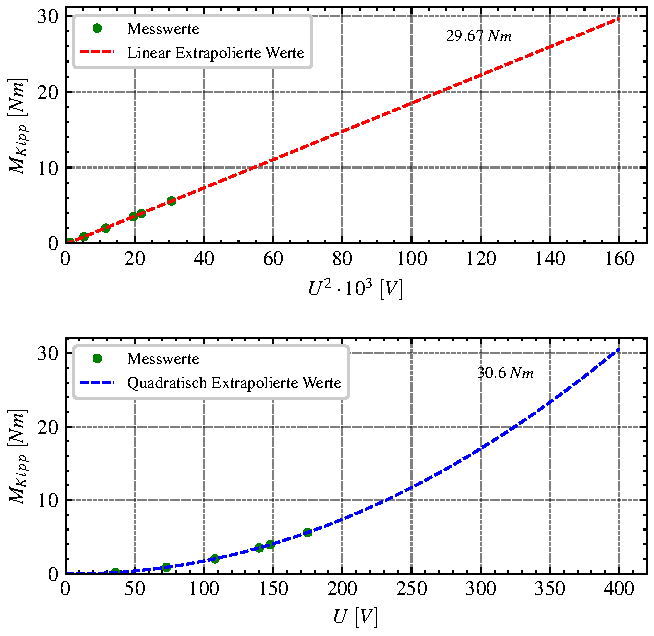
\includegraphics[width=\columnwidth]{./figures/kippmoment.pdf}
    \caption{Kippmoment}
    \label{fig:Kippmoment}
\end{figure}

Der lineare Verlauf in Abb.\ref{fig:Kippmoment}, $M_{\textit{Kipp}}(U)$ [\textcolor{red}{rot}]:
\begin{gather*}
    0,1863 x - 0,1431\\
    M_{Kipp}(U_N=400^2V^2)=29,67 \ \si{Nm}
\end{gather*}

Und die quadratische Polynomfunktion $M_{\textit{Kipp}}(U)$ [\textcolor{blue}{blau}]:
\begin{gather*}
    0,000198 x^2 - 0,0024495 x -0,035842\\
    M_{Kipp}(U_N=400V)=30,6\ \si{Nm}
\end{gather*}



\subsection{Zusammenhang zwischen Drehmoment und Spannung}

Bei zunehmender Spannung $U_1$ steigt das Drehmoment M quadratisch an. Das
Drehmoment ist direkt proportional zu $U^2$ ($M \sim U^2$) und darauf ergibt sich
folgende Beziehnung: \[ M = \textit{konst.} \cdot U \]


\section{Bestimmung der Ersatzschaltbildparameter}
\subsection{Parameterbestimmung aufgrund der Kurzschlussmessung}

Umrechnen der gemessenen Widerstandswerte auf die Bezugstemperatur $T=75^\circ$C :
\begin{align}
    R_{1_{75}} & = R_{1_{20}}\frac{235^\circ\si{C}+75^\circ\text{C}}{235^\circ\text{C}+20^\circ\text{C}}         \\
               & = 2,32\ \Omega\cdot \frac{235^\circ\si{C}+75^\circ\text{C}}{235^\circ\text{C}+20^\circ\text{C}} \\
    \label{eq:R1_75}
               & = 2,820\ \Omega
\end{align}

Berechnen des Läuferwiderstands mithilfe der Übersetzungsverhältnis:
\begin{align}
    R_2^\prime        & = \ddot{u}^2\cdot R_2 = 4,7^2 \cdot 216\si{m\Omega}   = 4,77 \Omega                       \\
    R_{2_{75}}^\prime & = R_{2_{20}}\frac{235^\circ\si{C}+75^\circ\si{C}}{235^\circ\si{C}+20^\circ\si{C}}         \\
                      & = 4,77\ \Omega\cdot \frac{235^\circ\si{C}+75^\circ\si{C}}{235^\circ\si{C}+20^\circ\si{C}} \\
    \label{eq:R_2^prime}
                      & = 5,8\ \Omega
\end{align}

Es gilt:
\begin{equation} \label{eq:Kurzschlusswiderstand_gemessen}
    \boxed{R_k = R_1 + R_2^\prime = 2,820\ \Omega + 5,8\ \Omega = 8,62\ \Omega}
\end{equation}

Aus der Kurzschlussmessung in 4.2.1 wird der Kurzschlusswiderstand $R_k$ mit:

\begin{equation} \label{eq:Kurzschlusswiderstand}
    \boxed{R_k = \frac{U_k}{I_k}\cdot cos\varphi_k}
\end{equation}

\begin{table}[htbp]
    \begin{tabularx}{\columnwidth}{XXXXX}
        \toprule
        $I_1[A]$ & $P_1[W]$ & $U[V]$ & $G[g]$ & $M_{an}[Nm]$ \\
        \midrule
        4,2      & 392      & 113    & 464    & 1,82074      \\
        \bottomrule
    \end{tabularx}
    \caption{Kurzschlussmessung 4.2.1}
    \label{tab:Kurzschlussmessung}
\end{table}

Mit den Werten aus der Tabelle \ref{tab:Kurzschlussmessung} kann $cos\varphi_k$
berechnet werden:

\begin{equation}
    \boxed{cos\varphi_k = \frac{P_1}{\sqrt{3} \cdot I_1 \cdot U}}
\end{equation}

\begin{equation} \label{eq:cosphi_solved}
    cos\varphi_k = \frac{392 \si{W}}{\sqrt{3} \cdot 4,2 \si{A} \cdot 113 \si{V}} = 0,4769
\end{equation}

Da die Maschine im Stern geschaltet ist, ergibt sich für die Spannung $U_k$:

\begin{equation} \label{eq:Uk_solved}
    \boxed{U_k = \frac{U}{\sqrt{3}}} = \frac{113 \si{V}}{\sqrt{3}} = 65,24 \si{V}
\end{equation}

In der Formel \ref{eq:Kurzschlusswiderstand} einsetzen:

\begin{equation} \label{eq:Kurzschlusswiderstand_calc}
    \boxed{R_k = \frac{65,24\si{V}}{4,2\si{A}}\cdot cos(61,51^\circ) = \underline{7,409 \Omega}}
\end{equation}

Die Streureaktanzen $X_{1\sigma}$ und $X_{2\sigma}^\prime$ werden mit:

\begin{equation} \label{eq:Streureaktanzen}
    X_{1\sigma} + X_{2\sigma}^\prime = \frac{U_k}{I_k}\cdot sin\varphi_k
\end{equation}

Da $X_{1\sigma} = X_{2\sigma}^\prime$ ist, ergibt sich:

\begin{align} \label{eq:Streureaktanzen_solved}
    \Aboxed{X_{1\sigma} & = X_{2\sigma}^\prime = \frac{U_k}{I_k}\cdot\frac{1}{2}\cdot sin\varphi_k} \\
                        & = \frac{65,24\si{V}}{3,69\si{A}}\cdot\frac{1}{2}\cdot sin(61,51^\circ)    \\
                        & =6,826\ \Omega
\end{align}

\subsubsection{Vergleich zwischen ermittelter und gemessener Kurzschlusswiderstand}

Die Werte des berechnete Kurzschlusswiderstands
(\ref{eq:Kurzschlusswiderstand_gemessen}) haben eine Abweichung von ca. 15 \% zu
dem gemessenen Widerstand (\ref{eq:Kurzschlusswiderstand_calc}). Diese Differenz
ist zu einem großen Teil auf die gewählte Referenztemperatur von 75°C zurück
zuführen. Bei einer zügig durchgeführten Messung ist die Wärmeentwicklung der
Maschine geringer. Nimmt man also einen geringeren Temperaturanstieg wie etwa
60°C an kommt man dem gemessenen Wert deutlich Näher.

\begin{equation}
    R_{2_{60}}^\prime = R_{2_{20}}^\prime \cdot \dfrac{60^\circ \si{C} + 235^\circ \si{C}}{20^\circ \si{C} + 235^\circ \si{C}}
\end{equation}

\begin{equation}
    R_{2_{60}}^\prime = 4,77 \Omega \cdot \dfrac{60^\circ \si{C} + 235^\circ \si{C}}{20^\circ \si{C} + 235^\circ \si{C}} = 4,77 \Omega
\end{equation}

aus (\ref{eq:Kurzschlusswiderstand_gemessen}):
\begin{equation}
    \boxed{R_{k} = R_{1} + R_{2_{60}}^\prime = 2,82 \Omega + 4,77 \Omega = 7,59 \Omega}
\end{equation}


\subsection{Parameterbestimmung aufgrund der Leerlaufmessung}
\subsubsection{Maschinenparameter $X_h$ und $R_{Fe+Reib}$ aufgrund der Leerlaufmessung}
Bei dem folgenden Versuch ist Läuferseitig ein Leerlauf und somit kein
Läuferstrom $I_{2}$ zu messen. Der fließende Strom besteht ausschließlich aus
dem Ständerstrom $I_{1}$ bzw. dem Magnetisierungsstrom $I_{0}$.
Der verwendete Hebelarm aus den letzten Messungen wird entfernt, der Läufer wird
mit kurzen Leitungen kurzgeschlossen.  Die verwendeten Werte werden Tabelle
\ref{tab:trennung_eisen_reib} entnommen.

Die gemessene Spannung wird auf die Strangspannung umgerechnet.
Anschließende wird über eine Masche der Spannungabfall $U_{h, Fe}$
berechnet.

\begin{equation}
    U_{Strang} = \dfrac{U}{ \sqrt{3} } = 230,94\si{V}
\end{equation}

\begin{align*}
    U_{h, Fe} & = U_{Strang} - U_{1} = U_{Strang} - R_{1} \cdot I_{0}        \\
              & = 230,94\si{V} - 2,32 \Omega \cdot 2,75\si{A} = 224,56\si{V}
\end{align*}


\begin{equation}
    \varphi_{0} = arcos\left( \dfrac{P_{0} - P_{Cu1} }{3 \cdot U_{Strang} \cdot I_{0} }\right) = 84,35^\circ
\end{equation}


\begin{align*}
    I_{Fe+Reib} & = I_{0} \cdot cos( \varphi ) = 0,27\si{A}   \\
    I_{m}       & = I_{0} \cdot sin( \varphi ) = 2,7367\si{A}
    %    Z_{h, Fe} = \dfrac{ U_{h, Fe} }{ I_{0} } = ( \frac{1}{X_{h}} + \frac{1}{R_{Fe}} )^{-1} = 81,66 \Omega
\end{align*}

\begin{equation}
    R_{Fe+Reib} = \dfrac{ U_{h, Fe} }{ I_{Fe+Reib} } = 831,7 \Omega
    %    \boxed{ R = Z_{h, Fe} \cdot ( \frac{1}{cos( \varphi) } +1 ) = 729,606 \Omega }
\end{equation}

\begin{equation}
    X_{h} = \dfrac{ U_{h, Fe} }{ I_{m} } = 82,06 \Omega
    %\boxed{ X_{h} = 91,95 \Omega }
\end{equation}

\subsubsection{Verhältniss aus Haupt- und Streureaktanz}

mit $X_{ \sigma } =  X_{1, \sigma } + X_{2, \sigma }^\prime$

\begin{equation}
    \dfrac{ X_{h}}{X_{ \sigma }} = \dfrac{ 82,06 \Omega }{ 13,652 \Omega } = 6,01
    %\dfrac{ X_{h}}{X_{ \sigma }} = \dfrac{ 91,95 \Omega }{ 13,652 \Omega } = 6,735
\end{equation}

Die Hauptreaktanz ist ca. 6 mal größer als die Streureaktanz.

\subsubsection{Vollständige Ersatzschaltbild [ESB]}
Das ESB beschreibt immer einen Strang der Maschine, so dass die Verschaltung
(Stern- oder Dreieck) bezüglich der Messgrößen Strom und Spannung zu
berücksichtigen ist. $U_1$ und $I_1$ stellen die Stranggrößen des
Ersatzschaltbildes dar.

\begin{figure}[htbp]
    \centering
    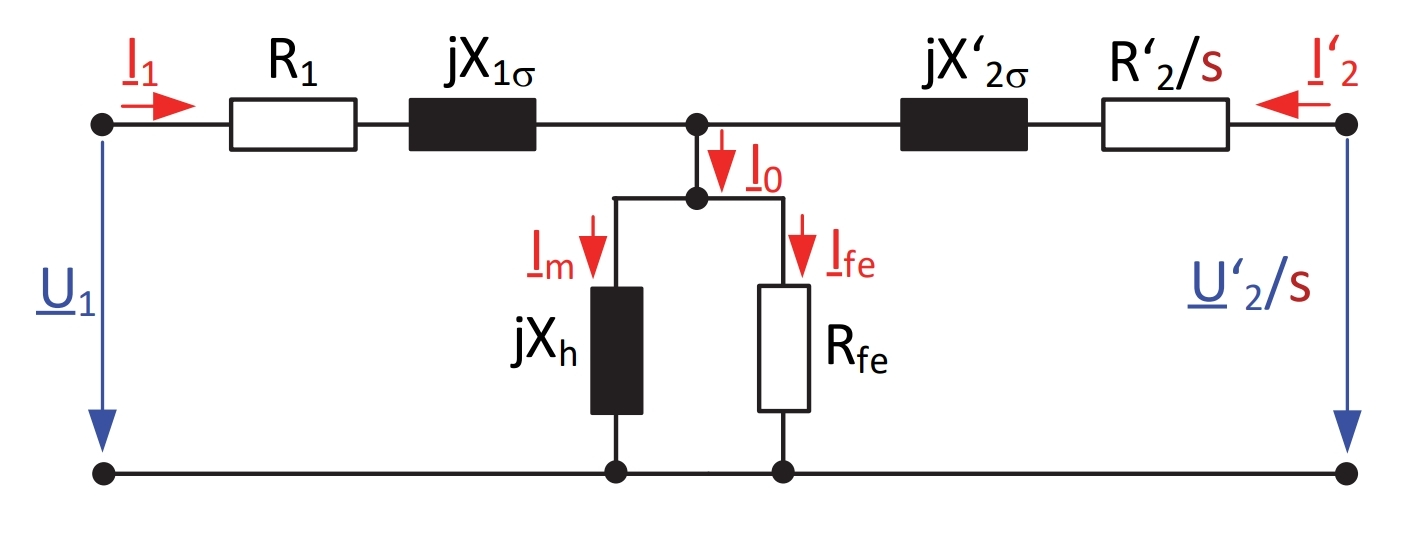
\includegraphics[width=\columnwidth]{./figures/Vollstaendiges_ESB.jpg}
    \caption{Vollständige Ersatzschaltbild}
    \label{fig:ESB_Vollstaendig}
\end{figure}

\section{Trennung von Eisen- und Reibungsverlusten}

Die gemessenen Leerlaufleistungen $P_{0}$ beinhalten $P_{Cu}$, $P_{Reib}$
und $P_{Fe}$. Um die Eisen- und Reibungsverluste zu trennen, werden als Erstes
die Kupferverluste$ P_{Cu}$ abgezogen.

\begin{equation}
    P_{0} - P_{Cu} = P_{Reib+Fe}
    \label{eq:P_reib_fe}
\end{equation}

\begin{table}[htbp]
    \centering
    \begin{tabularx}{\columnwidth}{XXXXXX}
        \toprule
        $I_0[A]$ &  $P_0[W]$ &  $P_{Cu}[W]$ &  $P_{Fe+Reib}$ &  $U[V]$ &  $n[min]$ \\
        & & & $[W]$& & \\
        \midrule
               2,75 &         240 &        19,1400 &            220,8600 &       400 &        1493 \\
               1,70 &         140 &        11,8320 &            128,1680 &       300 &        1490 \\
               1,10 &          80 &         7,6560 &             72,3440 &       200 &        1485 \\
               0,58 &          44 &         4,0368 &             39,9632 &       100 &        1461 \\
        \bottomrule
    \end{tabularx}
    \caption{Trennung von Eisen und Reibungsverlusten}
    \label{tab:trennung_eisen_reib}
\end{table}


Zur graphischen Ermittlung von $P_{Reib}$ werden die Messwerte für
$P_{Reib+Fe}$ nun graphisch als Funktion der quatratischen Spannung $U^2$
dargestellt.

\begin{figure}[htbp]
    \centering
    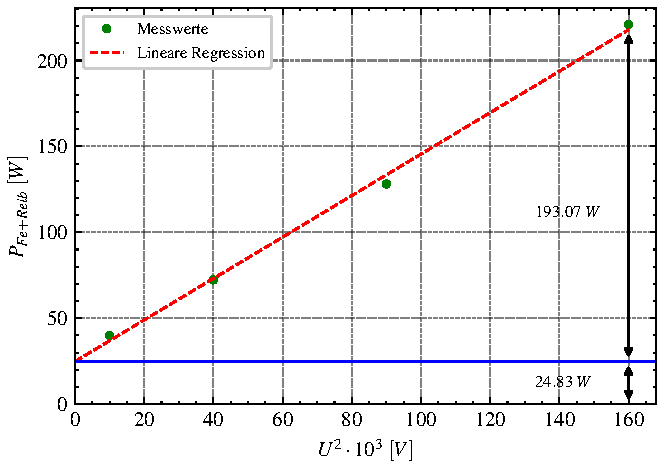
\includegraphics[width=\columnwidth]{./figures/trennung_eisen_reib.pdf}
    \caption{Trennung von Eisen- und Reibungsverlusten}
    \label{fig:trennung_von_eisen_reib}
\end{figure}

Die Messerwerte bilden eine Gerade, deren Ordinatenabschnitt $P_{Reib}$
darstellt. $P_{Reib} = 24,38 \si{W}$

Zur Berechnung von $R_{Reib}$ wird die Spannung, die ueber $R_{1}$ abfaellt zur
Vereinfachung vernachlaessigt.

\begin{equation}
    R_{Reib} = \dfrac{3\cdot U_{1N}^{2}}{ P_{Reib} } =
\end{equation}

Zur Bestimmung von $R_{Fe}$ wird $P_{Fe}$ an der Stelle $U_{1N}^{2}$ abglesen.
$P_{Fe} = 193,07 \si{W}$

\begin{equation}
    R_{Fe} = \dfrac{3\cdot U_{1N}^{2}}{ P_{Fe} } =
\end{equation}


\subsubsection{Parallelschaltung von $R_{Reib}$ und $R_{Fe}$}
\begin{equation}
    R_{Reib}||R_{Fe} = \dfrac{ R_{Reib} \cdot R_{Fe}}{R_{Reib} + R_{Fe}} =
\end{equation}

\subsubsection{Vergleich der Parallelschaltung von $R_{Reib}$ und $R_{Fe}$ mit $R_{Reib+Fe}$ aus 5.3.2}

\dots

\section{$M/n$ Kennlinie}

aus (\ref{eq:Streureaktanzen_solved}), (\ref{eq:R_2^prime}) und (\ref{eq:R1_75})

\smallskip
Mit $R_1 = 2,82\Omega$:
\begin{equation} \label{eq:s_k-mit-R_1}
    s_k = \frac{R_2^{\prime}}{\sqrt{R_{1}^{2} + X_{\sigma}^{2}}} = \frac{5,80\Omega}{\sqrt{2,82^2+13,652^2}\Omega} = 0,416
\end{equation}

\begin{align}
    M_{k} & = \frac{U_{1}^{2}}{4 \pi n_{1} \left(R_{1} + \sqrt{R_{1}^{2} + X_{\sigma}^{2}}\right)}           \\
          & = \frac{400\si{V}^{2}}{4 \pi \cdot 25 \si{sec^{-1}} \cdot (2,82 + \sqrt{2,82^2+13,652^2})\Omega} \\
          & = 31,653 \si{Nm}
    \label{eq:M_k-mit-R_1}
\end{align}

\smallskip
Mit $R_1 = 0\Omega$:
\begin{equation} \label{eq:s_k-naehrung}
    s_k \approx \frac{R_2^{\prime}}{X_{\sigma}} = \frac{5,80\Omega}{13,652\Omega} = 0,425
\end{equation}

\begin{align}
    M_{k} & \approx \frac{U_{1}^{2}}{4 \pi X_{\sigma} n_{1}} \approx \frac{400\si{V}^{2}}{4 \pi\cdot 13,652 \Omega \cdot 25 \si{sec^{-1}}} \\
          & \approx 37,306 \si{Nm}
    \label{eq:M_k-mit-R_1}
\end{align}

\begin{table}[htbp]
    \centering
    \begin{tabularx}{\columnwidth}{XXX}
        \toprule
        $s$   & $M[Nm]$ & $n_1[min^{-1}]$ \\
        \midrule
        -0,50 & -29,58  & 2250            \\
        -0,25 & -30,09  & 1875            \\
        0,00  & 0       & 1500            \\
        0,25  & 30,09   & 1125            \\
        0,50  & 29,58   & 750             \\
        0,75  & 24,01   & 375             \\
        1,00  & 19,49   & 0               \\
        \bottomrule
    \end{tabularx}
    \caption{Drehmoment über die Drehzahl}
    \label{tab:sigma_vs_M_n1}
\end{table}

\begin{table}[htbp]
    \centering
    \begin{tabularx}{\columnwidth}{XXXXXXX}
        \toprule
        $s$   & $M_{kipp}[Nm]$ & $n_1[min^{-1}]$ \\
        \midrule
        -0,50 & -25,32  & 2250            \\
        -0,25 & -14,90  & 1875            \\
        0,00  & 0       & 1500            \\
        0,25  & 14,90   & 1125            \\
        0,50  & 25,32   & 750             \\
        0,75  & 30,39   & 375             \\
        1,00  & 31,65   & 0               \\
        \bottomrule
    \end{tabularx}
    \caption{}
    \label{tab:M_kipp-mit-laeufervorwiderstand}
\end{table}


\begin{figure}[htbp]
    \centering
    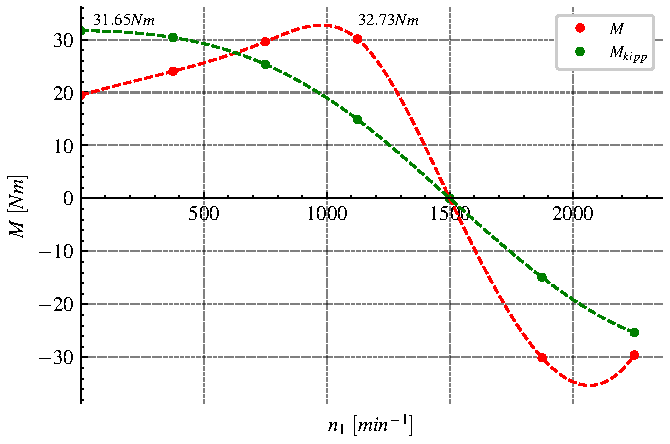
\includegraphics[width=\columnwidth]{./figures/m_n-kennlinie.pdf}
    \caption{$M/n$ Kennlinie}
    \label{fig:trennung_von_eisen_reib}
\end{figure}

\section{Wirkleistungsfluss}

\end{document}
